\section{Part B: Simulating the Penrose Process}
\label{Sec3}

\subsection{Kerr-Newman Metric}
For the final attempt, we are interested in the 4-dimensional rotating black hole and the investigation of the Penrose process. The metric of a 4-dimensional axisymmetric, stationary black hole in asymptotically flat spacetime is given by the Kerr-Newman solution,
\be\ba\label{Metric_Kerr-Newman}
	ds^2 = &-\frac{\Delta - a^2\sin^2\theta}{\Sigma}dt^2 + \frac{\Sigma}{\Delta}dr^2 + \Sigma d\theta^2 + \\
	&+ \frac{\left(r^2+a^2\right)^2 - a^2\Delta\sin^2\theta}{\Sigma}\sin^2\theta d\phi^2 - 2\frac{R_{S}ra\sin^2\theta}{\Sigma}dtd\phi
\ea\ee
with,
\be\ba
	\Delta &= r^2 + a^2 - R_{S}r + Q^2 \\
	\Sigma &= r^2 + a^2\cos^2\theta
\ea\ee
The parameters $R_{S}$, $a$ and $Q$ are the Schwarzschild radius, $R_{S}=2GM$, the spin parameter, $a=\frac{J}{M}$, with $J$ the angular momentum of the black hole around the $z$-axes, and the electric charge of the black hole respectively. This solution also has two event horizons,
\be
	r_{H}^{\pm} = \frac{R_{S}}{2}\left( 1 \pm \sqrt{1 - 4\frac{a^2 + Q^2}{R_{S}^2}} \right)
\ee
with only the outer horizon being physical, $r_{H} = r_{H}^{+}$.

Apart from the event horizons, the rotating black hole possesses a unique region, called the ergoregion. This is the region within which a particle cannot stay still and is given by the set of those points satisfying $g_{tt}>0$. As a result, the ergoregion is bounded by two ergospheres $r_{E}^{\pm}$ ( $r_{E}^{-} < r < r_{E}^{+}$),
\be
	r_{E}^{\pm} = \frac{R_{S}}{2}\left( 1 \pm \sqrt{1 - 4\frac{a^2\cos^2\theta + Q^2}{R_{S}^2}}  \right)
\ee
but only $r_{E}^{+} \equiv r_{E}$ is physical, while $r_{E}^{-} < r_{H}^{-}$ so, the real ergoregion is $r_{H}<r<r_{E}$.

\subsection{Penrose Process}
In 1971, Roger Penrose and R. M. Floyd (\cite{Penrose1971}) theorized the extraction of energy from a rotating black hole through a simple mechanism. The procedure is as in figure \ref{fig:PenroseProcess}. A parent particle (particle 1) with some energy $E_1$ decays into an outgoing particle (particle 2) with energy $E_2$ and an ingoing particle (particle 3) with energy $E_3$. Under special conditions, $E_3$ can be negative allowing particle 2 to be detected by a distant observer with an increased energy.

The condition for a negative energy is a $\phi$-component of the coordinate velocity smaller than a critical value,
\be\label{NES_vd}
	\upsilon^{\phi} < -\frac{g_{tt}}{g_{t\phi}}
\ee
This also sets an allowed range of the specific angular momentum $l\equiv\frac{L}{m}$,
\be\label{NES_l}
	l < -\sqrt{\frac{-\psi g_{\phi\phi}}{g_{t\phi}^2g_{tt}}}
\ee
where $\psi = g_{tt}g_{t\phi} - g_{t\phi}^2 = -\Delta\sin^2\theta <0 $ is the determinant of the sub-metric $2\times2$ matrix constructed only from $t$ and $\phi$ components,
\be
	\tilde{g} = \begin{pmatrix}
		g_{tt} & g_{t\phi} \\
		g_{\phi t} & g_{\phi\phi}
	\end{pmatrix}
	\Rightarrow \tilde{g}^{-1} = \frac{1}{\psi} \begin{pmatrix}
		g_{\phi\phi} & -g_{t\phi} \\
		-g_{\phi t} & g_{tt}
	\end{pmatrix}
\ee
From the specific angular momentum condition \eqref{NES_l}, it is obvious that the Penrose process can be produced only when $g_{tt}>0$, i.e. only within the ergoregion. The negative sign in \eqref{NES_l} also shows that the particle must have an opposite angular momentum ($L<0$) from the angular momentum of the black hole ($J>0$), while the $\phi$-component of the coordinate velocity can still be positive. Evidentially, a careful analysis of the process reveals that the extra energy particle 2 has gained comes from the rotational energy of the black hole; particle 3 is absorbed by the black hole lowering its total angular momentum to $J^{\prime} = J + L<J$.

\begin{figure}
	\centering
	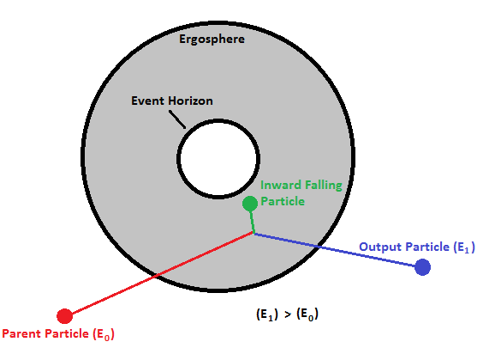
\includegraphics[height=8cm]{Figures/PenroseProcess.png}
	\caption[Mechanical Penrose Process]{Mechanical Penrose Process. A parent particle falls from infinity towards the black hole and decays into a new ingoing particle and an outgoing particle. The second in-falling particle can have negative energy within the ergoregion allowing the outgoing particle to be detected with increased energy from a distant observer.}
	\label{fig:PenroseProcess}
\end{figure}

At the point of split, conservation of 4-momentum must be satisfied,
\be
	p_{1\mu} = p_{2\mu} + p_{3\mu}
\ee
To simplify the problem, we consider equatorial motion, that is, we set $\theta = \frac{\pi}{2}$ and $\upsilon_1^{\theta} = \upsilon_2^{\theta} =\upsilon_3^{\theta} = 0$\footnote{It is simple to prove that, if the initial $\theta$-component of the coordinate velocity is zero at the equatorial plane, then it stays zero along the entire propagation. This follows from the conservation of the angular momentum $L$ which ensures that the motion is restricted to the plane perpendicular to $\vec{L} = L\hat{z}$}. In addition, to further simplify the simulation, we take $\upsilon_3^{r} = 0$. As a result, conservation of 4-momentum is expanded to the following 3 constraints,
\be\label{E_CONS}
	\epsilon_1 = \mu_2 \epsilon_2 + \mu_3 \epsilon_3 \Rightarrow \boxed{\epsilon_2 = \frac{\epsilon_1 - \mu_3 \epsilon_3}{\mu_2}}
\ee
\be\label{ur_CONS}
	\dot{t}_1 \upsilon_{1}^{r} = \mu_2 \dot{t}_2 \upsilon_{2}^{r} \Rightarrow \boxed{\upsilon_{2}^{r} = -\frac{\dot{t}_1\upsilon_{1}^{r}}{\mu_2}}
\ee
\be\label{L_CONS}
	l_1 = \mu_2 l_2 + \mu_3 l_3 \Rightarrow \boxed{l_{2} = \frac{l_1 - \mu_3 l_3}{\mu_2}}
\ee
where $\epsilon\equiv\frac{E}{m}$ and $l\equiv\frac{L}{m}$ are the specific energy and specific angular momentum respectively and $\mu_2$ and $\mu_3$ are the ratios of the masses of particles 2 and 3 over the mass of the parent particle, $\mu_2 \equiv \frac{m_2}{m_1}$, $\mu_3\equiv\frac{m_3}{m_1}$. In addition, we have a constraint following from $p^2 = -m^2$,
\be\label{M_CONS}
	p_2^2 = (p_1 - p_3)^2 = p_1^2 + p_3^2 - 2p_{1} \cdot p_{3} \Rightarrow \boxed{\mu_2 = \sqrt{1+\mu_3^2 + 2\mu_3 u_1 \cdot u_{3}}}
\ee

From these 4 equations, we can solve for $\upsilon_{2}^{r}$, $\upsilon_{2}^{\phi}$, $\mu_2$ and $\mu_3$ given the $\phi$-component of the coordinate velocity $\upsilon_{3}^{\phi}$ of particle 3. This is chosen to ensure that it has negative energy, that is, we take the splitting to take place within the ergoregion $r_{H}<r<r_{E}$ and $\upsilon_{3}^{\phi} < -\frac{g_{tt}}{g_{t\phi}}$.

To sum up so far, the known quantities are $\vec{\upsilon}_1 = (\upsilon_{1}^{r},0,\upsilon_{1}^{\phi})$ and $\vec{\upsilon}_3 = (0,0,\upsilon_{3}^{\phi})$, while the unknown quantities are $\vec{\upsilon}_2 = (\upsilon_{2}^{r},0,\upsilon_{2}^{\phi})$, $\mu_2$ and $\mu_3$.

Solving \eqref{ur_CONS}, we find that,
\be\label{v2r}
	\upsilon_{2}^{r} = \sqrt{-\frac{\lambda_1^2}{\lambda_1^2 g_{rr} + \mu_2^2}\left( g_{tt}+2g_{t\phi}\upsilon_{2}^{\phi} + g_{\phi\phi}(\upsilon_{2}^{\phi})^2 \right)}
\ee
where $\lambda_1 \equiv \dot{t}_1\upsilon_{1}^{r}$. We have chosen the ``$+$'' sign to ensure that particle 2 heads out and is not in danger of getting too close to the event horizon before escaping to infinity. Plugging this expression into the expression of $l_2 \equiv u_{2\phi}$ and using \eqref{L_CONS}, we find that,
\be
	\upsilon_{2}^{\phi} = g_{tt} \frac{-g_{t\phi} + \sqrt{-\psi}\sqrt{k(k+1)}}{g_{t\phi}^2 + kg_{tt}g_{\phi\phi}}
\ee
where the parameter $k$ is given by,
\be
	k = \left(\frac{\mu_3 l_3}{\mu_2}\right)^2\left(1-\frac{\lambda_1^2}{\lambda_1^2g_{rr}+\mu_2^2}\right)
\ee
Finally, use this result of $\upsilon_{2}^{\phi}$ to also write $\upsilon_{2}^{r}$ in terms of $\mu_2$ and $\mu_3$ and use \eqref{E_CONS} and \eqref{M_CONS} to solve for $\mu_2$ and $\mu_3$. This could in principle be done analytically but the calculations are too much so we instead be lazy and solve the system computationally using the Newton-Raphson method.

\subsection{Constraints on $\mu_2$ and $\mu_3$}
We can see that $\upsilon_{2}^{r}>0$ always exists\footnote{One could argue that $g_{tt}+2g_{t\phi}\upsilon_1^{\phi}+g_{\phi\phi}(\upsilon_{1}^{\phi})^2$ must be negative, but this follows directly from the fact that the particles are massive. This means that,
	\be\ba
		&-\dot{t}^{-2} = g_{tt} + 2g_{t\phi} + g_{rr}(\upsilon^{r})^2 + g_{\phi\phi}(\upsilon^{\phi})^2 < 0 \\
		&\Rightarrow g_{tt} + 2g_{t\phi} + g_{\phi\phi}(\upsilon^{\phi})^2 < -g_{rr}(\upsilon^{r})^2 < 0
	\ea\ee
given that the particle is outside the black hole ($r>r_{H}\Rightarrow g_{rr}>0$).}. The existence of $\upsilon_{2}^{\phi}$, however, requires that,
\be
	k(k+1) \ge 0 \Rightarrow k\ge0 \;\; or \;\; k\le-1
\ee
The first case of $k\ge0$ is always satisfied unless $g_{rr}\le1$ but that would require the particle to be inside the black hole\footnote{Expanding $g_{rr}\le1$ from \eqref{Metric_Kerr-Newman}, we find that $r\le\frac{a^2+Q^2}{R_{S}}$. Physical black holes are not naked singularities, meaning that the event horizon exists, i.e. $\frac{a^2+Q^2}{R_{S}}\le\frac{R_{S}}{4}$. Consequently, if $g_{rr}\le1$, then $r\le\frac{R_{S}}{4}$ but $\frac{R_{S}}{4}<r_{H}$.}. On the other hand, $k\le-1$ can never be achieved because it yields the condition,
\be
	\mu_3^2 \le \frac{\mu_2^2}{g_{tt}l_3^2} \frac{\lambda_1^2g_{rr} + \mu_2^2}{\lambda_1^2(1-g_{rr}) - \mu_2^2} < 0
\ee

The only true constraint on $\mu_2$ and $\mu_3$ is the requirement of particle 2 reaching infinity. This requires $\epsilon_2\ge1$ so,
\be
	\boxed{\mu_2 \le \epsilon_1 - \mu_3 \epsilon_3}
\ee

A natural process will also have $\mu_2^2 + \mu_3^2 < 1$ because,
\be
	p_1^2 = p_2^2 + p_3^2 + 2p_2 \cdot p_3 \Rightarrow \mu_2^2 + \mu_3^2 = 1 + 2p_2 \cdot p_3 < 1
\ee
since particles 2 and 3 are timelike-separated, i.e. $p_2 \cdot p_3 < 0$.

\subsection{Run 3: Results}
The rotating black hole we simulated has $J=0.9$ and $Q=0.0$. We firstly solved the geodesics using part A to simulate the propagation of the parent particle from very far $r = 100R_{S} = 200.0$ until somewhere near the black hole $r \sim r_{H} $. Then we used those values of $\{t,\vec{x},\vec{v}\}$ for the parent particle at $r\sim6.0$ as initial conditions to simulate the process. We propagated the parent particle until $r_{H} < r < r_{E}$ and then perform the splitting into particles 2 and 3 according to the above discussion.

The initial conditions for the parent particle were,
\begin{table}[H]
	\centering
	\begin{tabular}{|c|c|}
		\hline
		$t_{10}$ & 3176.535 \\
		\hline
		$r_{10}$ & 6.103719 \\
		\hline
		$\theta_{10}$ & $\frac{\pi}{2}$ \\
		\hline
		$\phi_{10}$ & 0.072048 \\
		\hline
		\hline
		$\upsilon_{1r0}$ & -0.386224 \\
		\hline
		$\upsilon_{1\theta0}$ & 0.0 \\
		\hline
		$\upsilon_{1\phi0}$ & 0.00769361 \\
		\hline
	\end{tabular}
	\caption[Run 3: Initial Conditions for parent particle]{Run 3: Initial Conditions for parent particle.}
	\label{tbl:RUN3_IC}
\end{table}

We set the final time instant to $t_{N}=3191.4575$ for which the final position for particle 1 and initial positions for particles 2 and 3 are,
\begin{table}[H]
	\centering
	\begin{tabular}{|c|c|}
		\hline
		$t_{02,3}$ & 3191.4425775 \\
		\hline
		$r_{02,3}$ & 1.72223189 \\
		\hline
		$\theta_{02,3}$ & $\frac{\pi}{2}$ \\
		\hline
		$\phi_{02,3}$ & 1.15216234 \\
		\hline
	\end{tabular}
	\caption[Run 3: Initial positions for particles 2 and 3]{Run 3: Initial positions for particles 2 and 3.}
	\label{tbl:RUN3_IC2}
\end{table}
After solving the equations for $\mu_3$, $\mu_2$ and the initial velocity for particle 2, we arrive at the following results,
\begin{table}[H]
	\centering
	\begin{tabular}{|c|c|}
		\hline
		$v_{2r0}$ & 0.08684806 \\
		\hline
		$v_{2\theta0}$ & 0.0 \\
		\hline
		$v_{2\phi0}$ & 0.22415412 \\
		\hline
		\hline
		$v_{3r0}$ & 0.0 \\
		\hline
		$v_{3\theta0}$ & 0.0 \\
		\hline
		$v_{3\phi0}$ & 0.09949532 \\
		\hline
	\end{tabular}
	\caption[Run 3: Initial velocities for particles 2 and 3]{Run 3: Initial velocities for particles 2 and 3.}
	\label{tbl:RUN3_IC3}
\end{table}
\begin{table}[H]
	\centering
	\begin{tabular}{|c|c|}
		\hline
		$\mu_2$ & $0.738561712$ \\
		\hline
		$\mu_3$ & $1.47921968 \cdot 10^{-5}$ \\
		\hline
	\end{tabular}
	\caption[Run 3: Masses of particles 2 and 3]{Run 3: Masses of particles 2 and 3.}
	\label{tbl:RUN3_IC4}
\end{table}

The specific energies of particles 1,2 and 3 are then,
\begin{table}[H]
	\centering
	\begin{tabular}{|c|c|}
		\hline
		$\epsilon_1$ & $0.994987723$ \\
		\hline
		$\epsilon_2$ & $1.37619187$ \\
		\hline
		$\epsilon_3$ & $-1.447716 \cdot 10^{3}$ \\
		\hline
	\end{tabular}
	\caption[Run 3: Specific energies of particles 1, 2 and 3]{Run 3: Specific energies of particles 1, 2 and 3.}
	\label{tbl:RUN3_IC5}
\end{table}

Finally, we solved the geodesics for particles 2 and 3 separately with final time instants $t_{2N}=5000.0$, $t_{3N}=3206.442575$ and number of time steps $N_2 = N_3 = 15000$. The relevant graphs are figures %\ref{fig:RUN3_xv} and \ref{fig:RUN3_U}.

\begin{figure}
	\centering
	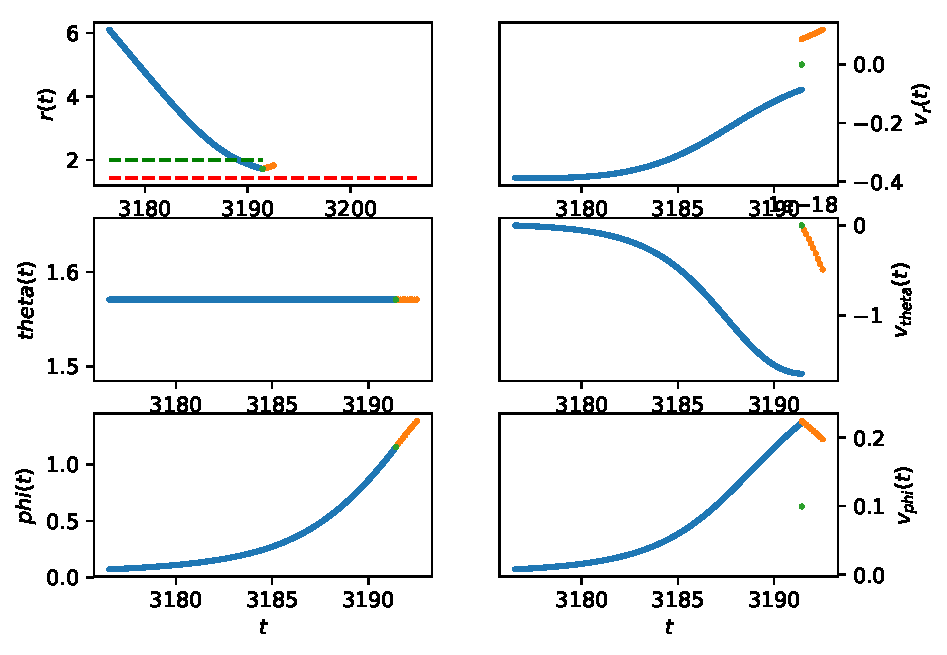
\includegraphics[height=8cm]{Figures/xv_t_Penrose.pdf}
	\caption[Run 3: Coordinate positions and velocities]{Run 3: Coordinate positions and velocities for the simulated Penrose process.}
	\label{fig:RUN3_xv}
\end{figure}

\begin{figure}
	\centering
	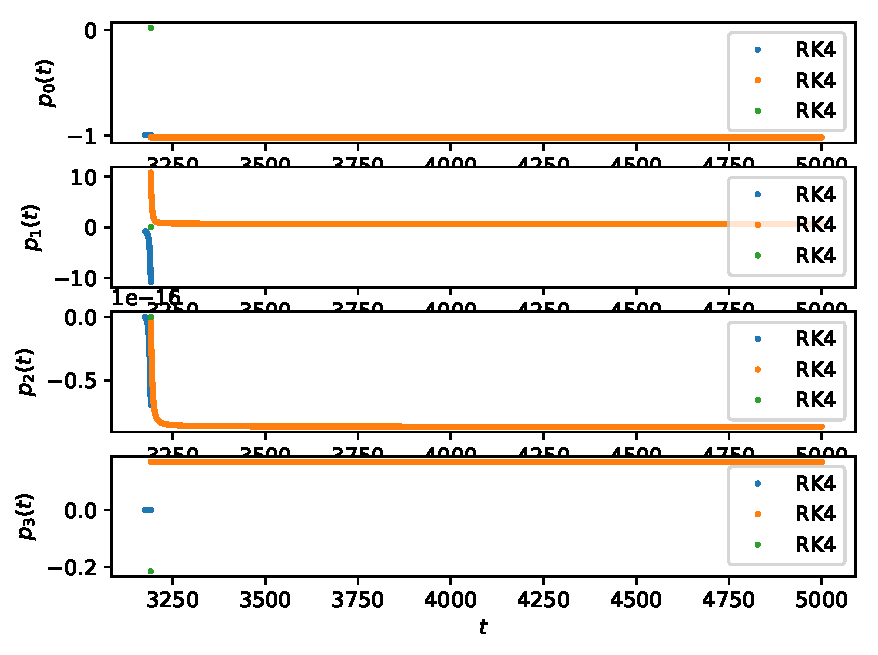
\includegraphics[height=8cm]{Figures/U_t_Penrose.pdf}
	\caption[Run 3: 4-momentum]{Run 3: 4-momentum for the simulated Penrose process.}
	\label{fig:RUN3_U}
\end{figure}